\chapter{Monitorowanie procesu gojenia ścięgna Achillesa}
\section{Ścięgno Achillesa}
Ścięgno Achillesa, nazywane również ścięgnem piętowym, jest największym i najsilniejszym ścięgnem występującym w ciele ludzkim. Stanowi wspólne zakończenie mięśnia trójgłowego łydki, w którego skład wchodzą dwie głowy mięśnia brzuchatego i mięsień płaszczkowaty. Całość struktury zlokalizowana jest w tylnym, powierzchownym przedziale łydki, co zostało przedstawione na Rysunku \ref{muscle_structure}.  
\begin{figure}[h!]
\centering
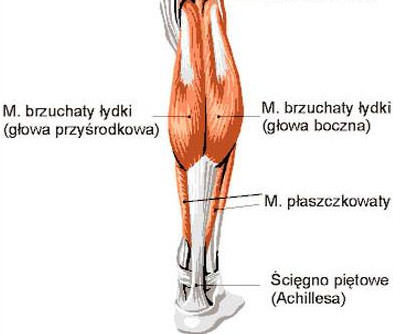
\includegraphics[width=0.55\textwidth]{figures/muscleStructure.jpg}
\caption{Lokalizacja mięśnia trójgłowego łydki wraz ze ścięgnem Achillesa.}
\label{muscle_structure}
\end{figure}
Z obu głów (brzuścców) mięśnia brzuchatego łydki wyrasta jedno szerokie, płaskie ścięgno, które jest początkiem części brzuchatej ścięgna Achillesa. Następnie ścięgno to łączy się z włóknami pochodzącymi od mięśnia płaszczkowatego, które układają się stycznie do wcześniej powstałej struktury. Wówczas kształt ulega stopniowemu zwężeniu i zaokrągleniu, aż do punktu o minimalnej szerokości (około 4 cm nad przyczepem dolnym [1]). W rejonie samego przyczepu dolnego znajdującego się na tylnej powierzchnia kości piętowej, ścięgno ponownie jest płaskie i szerokie.

W kolejnych podsekcjach szczegółowo omówiona została anatomia ścięgna Achillesa, jego biomechanika, potencjalne urazy wraz z czynnikami im sprzyjającymi oraz proces gojenia i możliwości jego wspomagania. Wszystkie te aspekty są istotne z uwagi na możliwości monitorowania procesów fizjologicznych występujących w ścięgnie. 
\subsection{Anatomia}
Średnia długość ścięgna Achillesa to 15 cm (11 - 26 cm). Średnia szerokość w rejonie początku wynosi 6.8 cm (4,5 - 8, 6 cm). Następnie, stopniowo ścięgno ulega zwężeniu do punktu o minimalnej szerokości 1.8 cm (1,2 - 2,6 cm). W rejonie samego przyczepu struktura ponownie się rozszerza i jej szerokość wynosi średnio 3.4 cm (2,0 - 4,8 cm) [2-3].
Zewnętrzną część ścięgna Achillesa stanowi ościęgno utworzone z tkanki łącznej włóknistej.
Achil
-Histologia
-Unaczynienie (krew, nerwy)

\subsection{Biomechanika}
Zadaniem ścięgien jest transfer siły mięśniowej do układu szkieletowego.
\subsection{Urazy i czynniki im sprzyjające}
\subsection{Leczenie, fazy gojenia i rehabilitacja}
\section{Zastosowanie rezonansu magnetycznego}
\section{Zastosowanie ultrasonografii}

Kolejną z metod obrazowania medycznego jest \textit{Ultrasonografia}, w skr. \textit{USG} (ang. \textit{Ultrasonography}, \textit{US}). Bazuje ona na efektach związanych z propagacją w tkankach \textit{ultradźwięków}, tj. fal akustycznych o częstotliwościach powyżej 20 kHz.

Propagacja fal w przyrodzie była tematem rozważań myślicieli takich jak Pitagoras, Arystoteles czy Galileusz, którzy ugruntowali pole badań pod kolejne osiągnięcia matematyczno-inżynieryjne. W tej kwestii, do jednego z przełomów doszło w 1822 roku, kiedy to szwajcarski inżynier Daniel Colladen oraz matematyk Charles-Francois Sturm wyznaczyli przybliżoną prędkość rozchodzenia się fali akustycznej w wodzie. Badanie wykonano na Jeziorze Genewskim, symultanicznie mierząc czas jaki potrzebny był dźwiękowi podwodnego wystrzału i sygnałowi dzwonka rozchodzącego się w powietrzu, aby przebyły drogę pomiędzy dwoma łódkami oddalonymi o 10 mil. Wyliczona wartość wyniosła wówczas 1435 m/s, nie różniąc się znacząco od dzisiaj przyjmowanej estymacji równej 1484 m/s. 

58 lat później, w 1880 roku bracia Curie opisali w \cite{Curie1880} \textit{efekt piezoelektryczny}, czyli zjawisko polegające na pojawieniu się ładunku elektrycznego pod wpływem naprężeń mechanicznych w krysztale o anizotropowej budowie, takiej jak ma np. kwarc. W przypadku odwrotnym, przyłożenie napięcia do odpowiedniego kryształu generuje drgania.


/*równanie dla głowicy*/ 
/*co mierzymy - oporność akustyczna, doppler*/
/*pole bliskie, dalekie*/
/*artefakty - snella odbicie, rozpraszanie, absorpcja i korygujący gain*/

Zalety: róŜnorodność informacji: obrazowanie w
czasie rzeczywistym, pomiary morfologiczne
i fizjologiczne
elastyczność zastosowań
niskie koszty
wykorzystanie bezpiecznego nośnika
informacji (niejonizującego) 

Dynamicznie rozwijająca się modalność
obrazowania
Powszechność zastosowań
Kompleksowa informacja diagnostyczna:
morfologia z badaniem funkcjonalnym
Podatność na nowe metody doskonalenia
efektów obrazowania

\section{Zastosowanie badań biomechanicznych}
\section{Inne metody}